\documentclass{article}
\usepackage{qilin}
\tikzstyle{process} = [rectangle, rounded corners, minimum width=1.5cm, minimum height=0.5cm,align=center, draw=black, fill=gray!30, auto]
\title{CHE260: Thermodynamics}
\author{QiLin Xue}
\date{Fall 2021}
\usepackage{mathrsfs}
\usetikzlibrary{arrows}
\begin{document}

\maketitle
\tableofcontents
\newpage
\section{Lecture 1}
\begin{idea}
    The three basic principles of engineering are:
    \begin{itemize}
        \item $F=ma$
        \item You can't push on a rope.
        \item A necessary condition for solving any given engineering problem is to know the answer before starting.
    \end{itemize}
\end{idea}
\section{Inelastic Behaviour}
\begin{itemize}
    \item Permanent deformation can be defined in three ways:
    \begin{enumerate}
        \item Upon unloading, sample does not return to original dimensions
        \item Strain does not return to zero
        \item Atoms move to new positions
        \item Occurs near the end of linear behaviour
    \end{enumerate}
    \item Plastic comes from the greek word \textit{plastikos}, which means to shape or to sculpt. In this course, plastic does not refer to the material type but instead the permanent deformation.
    \item The \textbf{strength} of a material describes when the permanent deformation occurs.
    \begin{warning}
        Strength depends on context and is not always defined as above.
    \end{warning}
    \item The stress strain curve for different materials resemble different shapes.
    \begin{itemize}
        \item Polymers have a distinct yielding region
        \item Metals start a concave down behaviour as soon as elastic deformation ends
        \item Ceramics have linear behaviour all the way until they fracture
    \end{itemize}
    \begin{figure}[ht]
        \centering
        \incfig{stress_strain}
    \end{figure}
    \item For polymers, the use of \textit{Young's Modulus} is misleading since the elastic behaviour depends on several different types of bonds, while Young's Modulus is related to the bahviour of a single bond. As a result, the term \textbf{elastic modulus} is used to describe polymers and composite materials.
    \subsection{Ceramics}
    \item Ceramics are not typically tested in tension because:
    \begin{enumerate}
        \item It is difficult to grip because it crumbles easily
        \item It is difficult to shape it into a dogbone shape
        \item Machine alignment is difficult to achieve.
    \end{enumerate}
    \item Instead, we test them by \textbf{3-point bending}:
    \begin{figure}[ht]
        \centering
        \incfig{3point_bending}
    \end{figure}
    \item The dotted line is the neutral axis and since it is weak in tension, the plate will break in the lower half at a stress value of:
    \begin{equation}
        \sigma = \frac{3FL}{2wh^2}
    \end{equation}
    \subsection{Tempered Glass}
    \begin{itemize}
        \item \textbf{Tempered glass} has a very high strength and is relatively ``safe'' when it fractures (small pieces instead of large ones)
        \begin{idea}
            Initially, tempered glass is very hot in a large volume. However, as it rapidly cools, the surfaces cool faster than the center. Since glass is made of silica bonded to four oxygen, it forms a very complex network structure. Therefore, during this rapid cooling, it ``fixes'' in excess volume.
            \vspace{2mm}
            
            The regions in the middle that are cooling more slowly is trying to contract but is constrained by the outer surface that it goes into tension. The fast cooling regions on the other hand will be in tension.
        \end{idea}
        \item When the glass bends, the opposite side of the window can still be in considerable compression even though for a regular ceramic it should be in tension. This increases the strength.
        \begin{figure}[ht]
            \centering
            \incfig{tempered_glass}
        \end{figure}
        \item The stress distribution creates \textbf{residual stress} which results in stored strain energy. When the glass gets fractured, the stored strain energy gets transformed into \textbf{surface energy}.
        \item Since surface energy is proportional to surface area, this means that the fractured pieces are smaller.
        \item \textbf{Chemical processes} can also be used to create tempered glass, usch as gorilla glass. Ions with a larger size diffuse into the surface and take up a larger space in the network resulting in an increase in volume at the surface.
    \end{itemize}
\end{itemize}
\section{Lecture 3 - Building Bridges}
\begin{itemize}
    \item Suppose we have a simple bridge over water:
    \begin{center}
        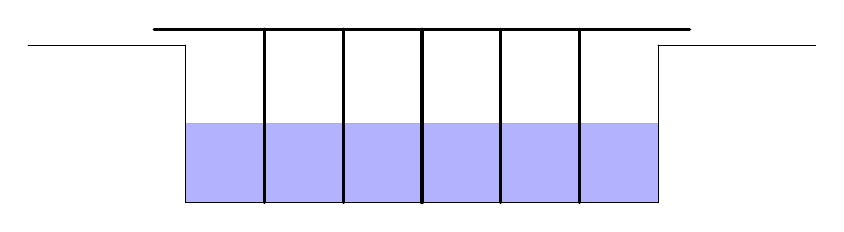
\begin{tikzpicture}[line cap=round,line join=round,>=triangle 45,x=1cm,y=1cm]
            
            \draw [fill=blue,opacity=0.3] (-3,1) rectangle (3,0);
            \draw [] (-5,2)-- (-3,2);
            \draw [] (-3,2)-- (-3,0);
            \draw [] (-3,0)-- (3,0);
            \draw [] (3,0)-- (3,2);
            \draw [] (3,2)-- (5,2);
            \draw [very thick] (-3.4,2.2)-- (3.4,2.2);
            \draw [very thick] (-2,2.2)-- (-2,0);
            \draw [very thick] (-1,0)-- (-1,2.2);
            \draw [very thick] (0,2.2)-- (0,0);
            \draw [very thick] (1,0)-- (1,2.2);
            \draw [very thick] (2,2.2)-- (2,0);
            \end{tikzpicture}
    \end{center}
    where the horizontal platform is known as the \textbf{beam} and the vertical supports are known as \textbf{posts} (which comes from the german word for tree)
    \item Disadvantages of this bridge is that it can easily break and become unusable in the event of a flood. This can be modified to become a \textbf{truss} bridge:
    \begin{center}
        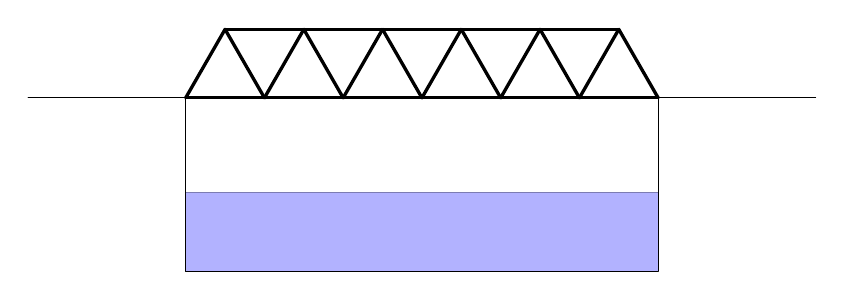
\begin{tikzpicture}[line cap=round,line join=round,>=triangle 45,x=1cm,y=1cm]
            \draw [fill=blue,opacity=0.3] (-3,1) rectangle (3,0);
            \draw [] (-5,2.2)-- (-3,2.2);
            \draw [] (-3,2.2)-- (-3,0);
            \draw [] (-3,0)-- (3,0);
            \draw [] (3,0)-- (3,2.2);
            \draw [] (3,2.2)-- (5,2.2);
            \draw [very thick] (-3,2.2)-- (3,2.2);

            \foreach \x in {-3,-2,...,2}
            \draw [very thick] (\x ,2.2)-- (0.5+\x ,3.07);

            \foreach \x in {-3,-2,...,2}
            \draw [very thick] (\x+1,2.2)-- (0.5+\x ,3.07);

            \draw [very thick] (-2.5,3.07) -- (2.5,3.07);
            \end{tikzpicture}
    \end{center}
    However this type of bridge needs constant maintenance and none of the truss bridges the Romans have built lasted to today.
    \item One of the oldest bridges (est. 5000 BC) was built across a large pond, known as the ``Sweet Track.'' The bridge was built in an X-shape and people could walk on top:
    \begin{center}
        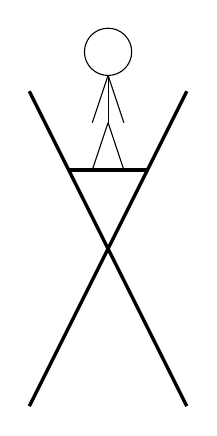
\begin{tikzpicture}
            \draw [very thick] (-1,2)-- (1,-2);
            \draw [very thick] (-1,-2)-- (1,2);
            \draw [] (0,2.2)-- (0,1.6);
            \draw [] (0,2.5) circle (0.3cm);
            \draw [very thick] (-0.5,1)-- (0.5,1);
            \draw [] (0,1.6)-- (-0.2,1);
            \draw [] (0,1.6)-- (0.2,1);
            \draw [] (0,2.2)-- (-0.2,1.6);
            \draw [] (0,2.2)-- (0.2,1.6);
        \end{tikzpicture}
    \end{center}
    \item Another form of bridge is suspended by hanging chains, known as a \textbf{suspension bridge}. A strong \textit{main cable} is pulled over two towers and fixed into concrete supports. Secondary \textit{hanging cables} run vertically and add support to the bridge.
    \begin{center}
        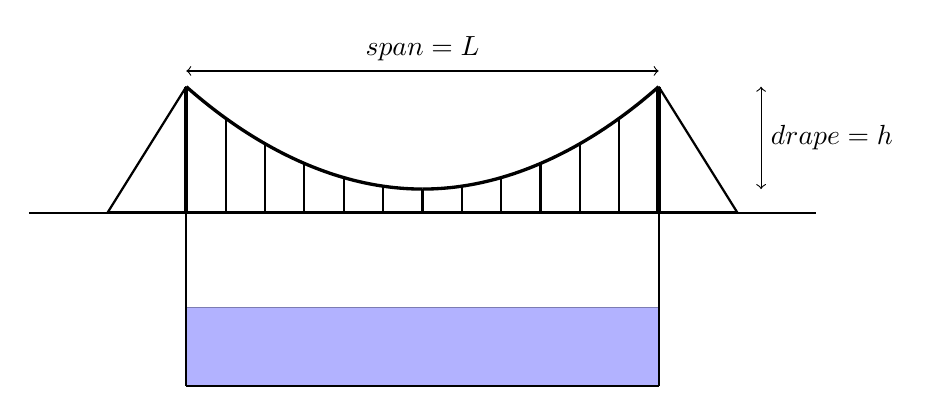
\begin{tikzpicture}
            \draw [fill=blue,opacity=0.3] (-3,1) rectangle (3,0);
            \draw [thick] (-5,2.2)-- (-3,2.2);
            \draw [thick] (-3,2.2)-- (-3,0);
            \draw [thick] (-3,0)-- (3,0);
            \draw [thick] (3,0)-- (3,2.2);
            \draw [thick] (3,2.2)-- (5,2.2);
            
            \draw [very thick] (0,2.5) parabola (3,3.8);
            \draw [very thick] (0,2.5) parabola (-3,3.8);
            \draw [very thick] (-4,2.2)-- (4,2.2);

            \foreach \x in {-2.5,-2,...,2.5}
            \draw [thick] (\x ,2.2)-- (\x ,0.144*\x*\x+2.5);

            \draw [ultra thick] (-3 ,2.2)-- (-3,3.8);
            \draw [thick] (-4,2.2) -- (-3,3.8);
            \draw [ultra thick] (3 ,2.2)-- (3,3.8);
            \draw [thick] (4,2.2) -- (3,3.8);
          
            \draw [<->] (-3,4) -- (3,4) node[midway,above] {$\text{span}=L$};
            \draw [<->] (4.3,2.5) -- (4.3,3.8) node[midway,right] {$\text{drape}=h$};
        \end{tikzpicture}
    \end{center}
    The ratio of the drape to the span is very important in determining how well the bridge is able to support the load. A typical ratio would be $L:h=10:1$.
    \item The \textbf{dead load} refers to the weight of the bridge as is, and the \textbf{live load} refers to the actual cars and people that need to cross the bridge. 
    \item Under its own weight or under a constant force, a piece of rope or flexible material will form the shape of a \textbf{catenary}, which is a shape that minimizes the potential energy of the system.
    \item The \textbf{catenary} shape very closely resembles that of a parabola, at least for small enough values, such that for most purposes it can be approximated as such.
\end{itemize}
\section{Crystallographic Planes and Directions}
\begin{itemize}
    \item We develop a set of notation to describe directions. It comes with a set of rules:
    \begin{itemize}
        \item Translate vector, if it simplifies things.
        \item Determine projection onto $x$, $y$, $z$.
        \item Reduce to lowest integers.
        \item Enclose in square brackets (negative signs are moved above, no commas)
    \end{itemize}
    \begin{example}
        We can find the crystallographic directions of both the blue and the red vectors in the figure below.
        \begin{center}
            \incfig{crystallographic_intro}
        \end{center}
        For the blue vector, we first let the tail by the origin. The vector travels $1$ in the negative $x$ direction, $0$ in the $y$ direction, and $-1$ in the negative $z$ direction, which gives $[\bar{1}\,0\,\bar{1}]$.
        \vspace{2mm}

        For the red vector, it travels in the negative $y$ direction for $0.5$ and in the negative $z$ direction for $1$ so we get, after getting rid of fractions: $[0\,\bar{1}\,\bar{2}]$.
    \end{example}
    \item To denote a family of directions, we can use braket notation. All face diagonals can be written as:
    \begin{equation}
        <0\,1\,1>
    \end{equation}
    which includes:
    \begin{equation}
        [0\,1\,1],\, [0\,\bar{1}\,1],\, [0\,1\,\bar{1}],\, [1\,0\,1], \ddots
    \end{equation}
\end{itemize}
\end{document}